% Created 2021-06-06 Sun 00:54
% Intended LaTeX compiler: pdflatex
\documentclass[11pt]{article}
\usepackage[utf8]{inputenc}
\usepackage[T1]{fontenc}
\usepackage{xcolor}
\usepackage{hyperref}
\usepackage[top=1in, bottom=1.25in, left=1.25in, right=1.25in]{geometry}
\usepackage{amsmath}
\usepackage[style=ieee,hyperref=true,backref=true,url=true,backend=biber,natbib=true]{biblatex}
\addbibresource{ref.bib}
\usepackage{chessboard}
\ExplSyntaxOn %requires texlive 2020, in older system load expl3
\cs_new:Npn \getfieldnumber #1
{
\fp_eval:n { (\tl_tail:V #1 -1)*8 + \exp_args:Ne\int_from_alph:n{\tl_head:V #1} -1}
}
\ExplSyntaxOff
\usepackage{titlesec}
\setcounter{secnumdepth}{4}
\titleformat{\paragraph}
{\normalfont\normalsize\bfseries}{\theparagraph}{1em}{}
\titlespacing*{\paragraph}
{0pt}{3.25ex plus 1ex minus .2ex}{1.5ex plus .2ex}

% features: (embed-files embed-tangled acronym underline par-sep image float-wrap engraved-code-setup engraved-code)

  \usepackage[main,include]{embedall}
  \IfFileExists{./\jobname.org}{\embedfile[desc=The original file]{\jobname.org}}{}
  


\newcommand{\acr}[1]{\protect\textls*[110]{\scshape #1}}
\newcommand{\acrs}{\protect\scalebox{.91}[.84]{\hspace{0.15ex}s}}
\usepackage[normalem]{ulem}
\setlength{\parindent}{0pt}

\usepackage{graphicx}
\usepackage{wrapfig}

  \usepackage{fvextra}
  \fvset{
    commandchars=\\\{\},
    highlightcolor=white!95!black!80!blue,
    breaklines=true,
    breaksymbol=\color{white!60!black}\tiny\ensuremath{\hookrightarrow}}
  \renewcommand\theFancyVerbLine{\footnotesize\color{black!40!white}\arabic{FancyVerbLine}}

  \definecolor{codebackground}{HTML}{f7f7f7}
  \definecolor{codeborder}{HTML}{f0f0f0}

  % TODO have code boxes keep line vertical alignment
  \usepackage[breakable,xparse]{tcolorbox}
  \DeclareTColorBox[]{Code}{o}%
  {colback=codebackground, colframe=codeborder,
    fontupper=\footnotesize,
    colupper=EFD,
    IfNoValueTF={#1}%
    {boxsep=2pt, arc=2.5pt, outer arc=2.5pt,
      boxrule=0.5pt, left=2pt}%
    {boxsep=2.5pt, arc=0pt, outer arc=0pt,
      boxrule=0pt, leftrule=1.5pt, left=0.5pt},
    right=2pt, top=1pt, bottom=0.5pt,
    breakable}
  
\definecolor{EFD}{HTML}{383a42}
\newcommand{\EFD}[1]{\textcolor{EFD}{#1}} % default
\definecolor{EFk}{HTML}{e45649}
\newcommand{\EFk}[1]{\textcolor{EFk}{#1}} % font-lock-keyword-face
\definecolor{EFd}{HTML}{84888b}
\newcommand{\EFd}[1]{\textcolor{EFd}{\textit{#1}}} % font-lock-doc-face
\definecolor{EFt}{HTML}{986801}
\newcommand{\EFt}[1]{\textcolor{EFt}{#1}} % font-lock-type-face
\definecolor{EFs}{HTML}{50a14f}
\newcommand{\EFs}[1]{\textcolor{EFs}{#1}} % font-lock-string-face
\definecolor{EFw}{HTML}{986801}
\newcommand{\EFw}[1]{\textcolor{EFw}{#1}} % font-lock-warning-face
\definecolor{EFb}{HTML}{a626a4}
\newcommand{\EFb}[1]{\textcolor{EFb}{#1}} % font-lock-builtin-face
\definecolor{EFct}{HTML}{9ca0a4}
\newcommand{\EFct}[1]{\textcolor{EFct}{#1}} % font-lock-comment-face
\definecolor{EFc}{HTML}{b751b6}
\newcommand{\EFc}[1]{\textcolor{EFc}{#1}} % font-lock-constant-face
\definecolor{EFpp}{HTML}{4078f2}
\newcommand{\EFpp}[1]{\textcolor{EFpp}{\textbf{#1}}} % font-lock-preprocessor-face
\definecolor{EFnc}{HTML}{4078f2}
\newcommand{\EFnc}[1]{\textcolor{EFnc}{\textbf{#1}}} % font-lock-negation-char-face
\definecolor{EFv}{HTML}{6a1868}
\newcommand{\EFv}[1]{\textcolor{EFv}{#1}} % font-lock-variable-name-face
\definecolor{EFf}{HTML}{a626a4}
\newcommand{\EFf}[1]{\textcolor{EFf}{#1}} % font-lock-function-name-face
\definecolor{EFcd}{HTML}{9ca0a4}
\newcommand{\EFcd}[1]{\textcolor{EFcd}{#1}} % font-lock-comment-delimiter-face
\definecolor{EFrc}{HTML}{4078f2}
\newcommand{\EFrc}[1]{\textcolor{EFrc}{\textbf{#1}}} % font-lock-regexp-grouping-construct
\definecolor{EFrb}{HTML}{4078f2}
\newcommand{\EFrb}[1]{\textcolor{EFrb}{\textbf{#1}}} % font-lock-regexp-grouping-backslash
\newcommand{\EFob}[1]{#1} % org-block
\definecolor{EFhn}{HTML}{da8548}
\newcommand{\EFhn}[1]{\textcolor{EFhn}{\textbf{#1}}} % highlight-numbers-number
\definecolor{EFhq}{HTML}{4078f2}
\newcommand{\EFhq}[1]{\textcolor{EFhq}{#1}} % highlight-quoted-quote
\definecolor{EFhs}{HTML}{986801}
\newcommand{\EFhs}[1]{\textcolor{EFhs}{#1}} % highlight-quoted-symbol
\definecolor{EFrdi}{HTML}{4078f2}
\newcommand{\EFrdi}[1]{\textcolor{EFrdi}{#1}} % rainbow-delimiters-depth-1-face
\definecolor{EFrdii}{HTML}{a626a4}
\newcommand{\EFrdii}[1]{\textcolor{EFrdii}{#1}} % rainbow-delimiters-depth-2-face
\definecolor{EFrdiii}{HTML}{50a14f}
\newcommand{\EFrdiii}[1]{\textcolor{EFrdiii}{#1}} % rainbow-delimiters-depth-3-face
\definecolor{EFrdiv}{HTML}{da8548}
\newcommand{\EFrdiv}[1]{\textcolor{EFrdiv}{#1}} % rainbow-delimiters-depth-4-face
\definecolor{EFrdv}{HTML}{b751b6}
\newcommand{\EFrdv}[1]{\textcolor{EFrdv}{#1}} % rainbow-delimiters-depth-5-face
\definecolor{EFrdvi}{HTML}{986801}
\newcommand{\EFrdvi}[1]{\textcolor{EFrdvi}{#1}} % rainbow-delimiters-depth-6-face
\definecolor{EFrdvii}{HTML}{4db5bd}
\newcommand{\EFrdvii}[1]{\textcolor{EFrdvii}{#1}} % rainbow-delimiters-depth-7-face
\definecolor{EFrdiix}{HTML}{80a880}
\newcommand{\EFrdiix}[1]{\textcolor{EFrdiix}{#1}} % rainbow-delimiters-depth-8-face
\definecolor{EFrdix}{HTML}{887070}
\newcommand{\EFrdix}[1]{\textcolor{EFrdix}{#1}} % rainbow-delimiters-depth-9-face
% end features
\author{Jake Moss - s46409665}
\date{\today}
\title{Chess game animation in blender}
\hypersetup{
 pdfauthor={Jake Moss - s46409665},
 pdftitle={Chess game animation in blender},
 pdfkeywords={},
 pdfsubject={},
 pdfcreator={Emacs 28.0.50 (Org mode 9.5)}, 
 pdflang={English}}
\begin{document}

\maketitle
\tableofcontents

\newpage

\section{Introduction}
\label{sec:orgeb540e2}
\subsection{Project aims}
\label{sec:org8c9b236}
This project aims to demonstrate a sufficient knowledge of computer graphics
techniques and implementations through the creation of a visually appealing
chess game animation tool. This was accomplished using Blender, and its python
scripting API.

This project utilises two tools to create the chess animation
\begin{itemize}
\item Blender\\
Blender had a large appeal due to is its extensibility through \texttt{Python} for
this project The exposed API allows its users to  script typical actions, and develop add-ons in a familiar
and standard environment. Part of this scripting API allows the user to add
and remove objects, insert key-frames, and change the properties of an object,
anything a user can do with a mouse and keyboard, is able to be configured
programmatically. This allows Blender to be used a front end to any \texttt{Python}
or \texttt{C++} program.
\item \texttt{python-chess} library\\
The \texttt{python-chess} library is a chess library for python with move validation,
generation, and \texttt{PGN} (Portable Game Notation, the most common file format
for chess games) parsing. This library is designed to be able to function as
back-end, making it perfect to use in conjunction with Blender.
\end{itemize}
\section{The plan}
\label{sec:org18ad456}
During the proposal the plan was to create an interactive, real time chess
board, however this was changed as the techniques and concepts would be severely
limited. Blender with python scripting was a perfect compromise.
\section{Blender implementation}
\label{sec:org30482dc}
\subsection{Modelling, textures, and shading}
\label{sec:org6f96ff1}
The scaling of the models was deliberately chosen to be unrealistic in order to
simplify the translation from position with the back to front end (See \hyperref[sec:org789c6c4]{Python
side - Array index to world space})
\subsubsection{Nodes}
\label{sec:orga47842b}
Blender nodes allow for the creation of textures and shaders through a pipeline
of simple operations to create complex procedural results. Its simple to
understand visual workflow is a popular alternative to layer based compositing.
\cite{node-vs-layer}

Throughout this project, procedural texture and shading generation using nodes
was used instead of the traditional texture wrapping using UV mapping in order
to give objects consistent and appealing surfaces. This provides two relevant
benefits;
\begin{itemize}
\item Tweaking textures and shading doesn't require an any more work than changing
values on the respective node.
\item Textures can be applied to any model without fitting issues, i.e. repetition
and resolution.
\end{itemize}
\subsubsection{Shaders}
\label{sec:org3b0d7af}
A shader is a program, typically run on the GPU, to computer the colour of a
group or individual pixel. These shaders describe the lighting interactions of
objects or surfaces, such as reflection, refractions, and absorption.
\paragraph{Principled BSDF}
\label{sec:orge816ad1}
A \texttt{BSDF} (Bidirectional Scattering Distribution Function) describes how light
scatters on a surface. In computer graphics, computing a highly detailed
microsurface is not feasible, instead it is replaced with a simplified
macrosurface (See Figure \ref{micro-vs-macro}). As the surface no longer retains the
detail it would in reality, light behaves differently on this new macrosurface.
To compensate for this a \texttt{BSDF} is used that matches the aggregate direction
scattering of the microsurface (at distance). \cite{ggx-paper}
\begin{figure}[htbp]
\centering
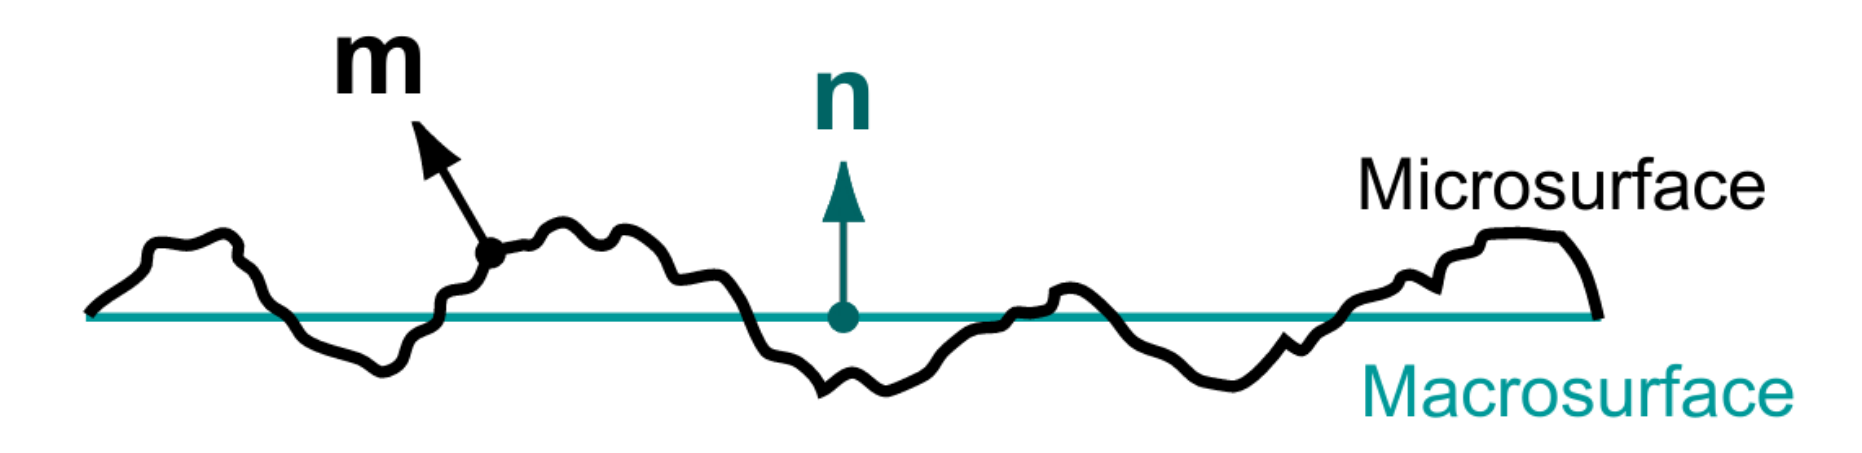
\includegraphics[width=0.5\textwidth]{Images/macro vs micro.png}
\caption{\label{micro-vs-macro}Micro vs macro surface \href{https://www.cs.cornell.edu/\~srm/publications/EGSR07-btdf.pdf}{(Source)}}
\end{figure}

Blenders implementation breaks down this problem down into two separate functions
by assuming that the microsurface can be adequately described using a microfacet
distribution function and a shadowing-masking function.

Blender provides these options for the distribution and shadowing functions, and
the subsurface methods.
\begin{itemize}
\item Distribution\footnote{Note that the \texttt{Distrubution} option Blender gives is different from the
\texttt{Microfacet Distrubution Function}, and includes both the \texttt{MDF} and the
Shadow-masking function.}
\begin{itemize}
\item GGX \\
\texttt{GGX} is a \texttt{BRDF} (bidirectional reflection distribution function) which
aims to be a faster than its alternative \texttt{Multiple-scattering GGX} at the
cost  of physical accuracy.
The \texttt{MDF} describes the distribution of microsurface normals \textbf{m} (Figure
\ref{micro-vs-macro}) while the shadow masking function describes what fraction of
the microsurface normals \textbf{m} are visible. \cite{ggx-paper}

In \texttt{GGX} the shadow masking function does not account for reflections or
scattering. This can create excessive darkening and a loss in energy
conservation in some areas \cite{principled-bsdf-docs}.

\item Multiple-scattering GGX \\
Almost all popular parametric \texttt{BSDF}'s only consider single reflection
to account for self-shadowing but omit outgoing light that scatters
multiple times between microfacets. Omitting outgoing light  breaks
conservation of energy and leads to dark patches within rough surfaces
\cite{ms-ggx-paper}.
\begin{figure}[htbp]
\centering
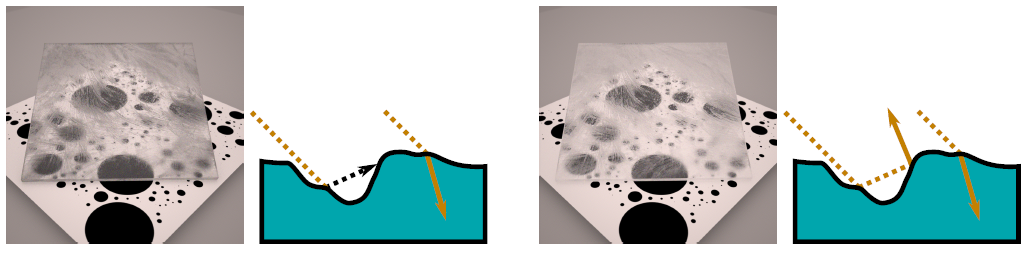
\includegraphics[width=.9\linewidth]{Images/multiplescatteringsmith_teaser.png}
\caption{Single scattering (left), multiple scatters (right), \href{https://eheitzresearch.files.wordpress.com/2015/10/multiplescatteringsmith\_teaser.png}{(Source)}}
\end{figure}

Blenders \texttt{Multiple-scattering GGX} \texttt{BRDF} allows for multiple light bounces
within microfacets to achieve 100\% energy conservation and provide a more
physically accurate render \cite{principled-bsdf-docs,ms-ggx-paper} . It
accomplishes this by conducting a random walk on the microsurface until the
ray escapes. Unlike \texttt{GGX} there is no known analytical expression for this
model (Blender's specific implementation), it must instead be solved
stochastically \cite{blender-issue-tracker}.
This comes at a performance cost, the original papers cites a 19\% penalty
using a Monte Carlo physically based renderer, Blenders development forums
estimates the performance penalty to be approximately 3\% at the time of
implementation \cite{blender-issue-tracker}.
\end{itemize}

\item Subsurface Scattering Method
Subsurface scattering when light passes through an object that is normally
opaque. Described by a \texttt{BSSRDF} (bidirectional subsurface scattering
reflectance distribution function)
\begin{itemize}
\item Christensen-Burley \\
The \texttt{Chistensen-Burley} method is an approximation of a physically based
volumetric scattering system with faster evaluation and efficiency \cite{Christensen-Burley}.
TODO
\item Random walk \\
\ldots{}
This comes at a cost of rendering time (actually performance hit is largely
dependent on the model itself), and increased noise.
TODO
\end{itemize}
\end{itemize}


All renders within this report have \texttt{Multiple-scattering GGX} enabled as the
benefit was need to outweigh the cost.

The \texttt{Principled BSDF} shader is a combination of multiple layers into a single
node. This is done for ease of use.

This shader encapsulates bidirectional reflectance and transmittance
distribution functions. Individually these functions determine how light behaves
on the surface and inside a material.


\subsubsection{Pieces}
\label{sec:orgd2bb58b}
Pieces were modelled after the reference image below Figure \ref{piece-reference}.
From this image the pieces where traced using the \texttt{Add Vertex} tool, from the
\href{https://docs.blender.org/manual/en/2.92/addons/add\_mesh/mesh\_extra\_objects.html}{Add Mess Extra Objects} add-on. To transform this line of vertices to a solid
object  a \texttt{Screw} modifier was applied.
\begin{figure}[htbp]
\centering
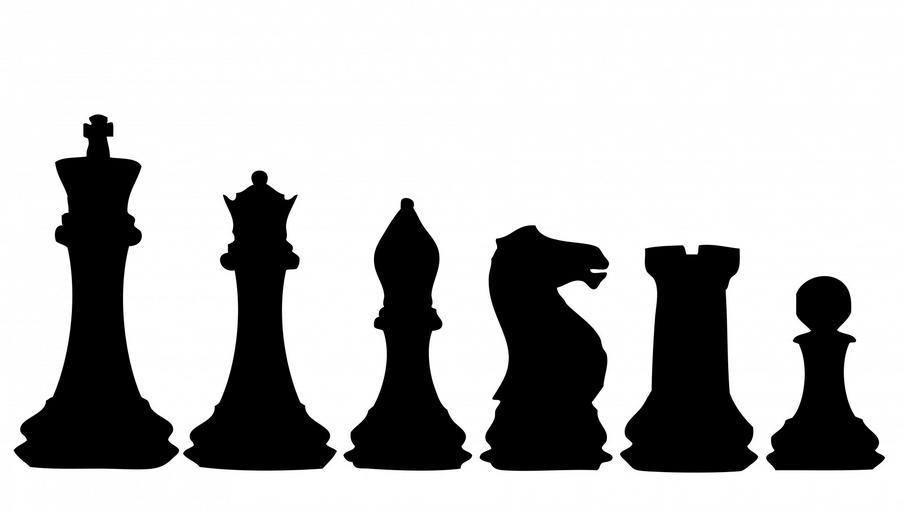
\includegraphics[width=0.5\textwidth]{ref/bee5aa3d08a30da4ca1005cbd0fe10b54a03bb49.jpg}
\caption{\label{piece-reference}Reference image, Licensed under \href{https://pixabay.com/service/license/}{Pixabay License}}
\end{figure}

\begin{center}
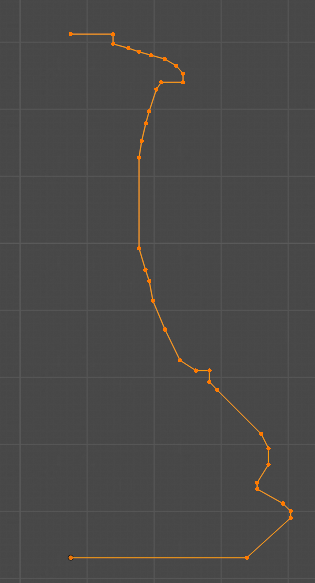
\includegraphics[height=150pt]{Images/modelling piece inprogress.png}
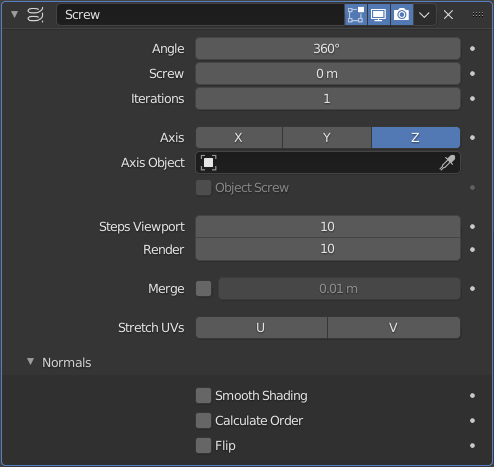
\includegraphics[height=150pt]{Images/screw settings.png}
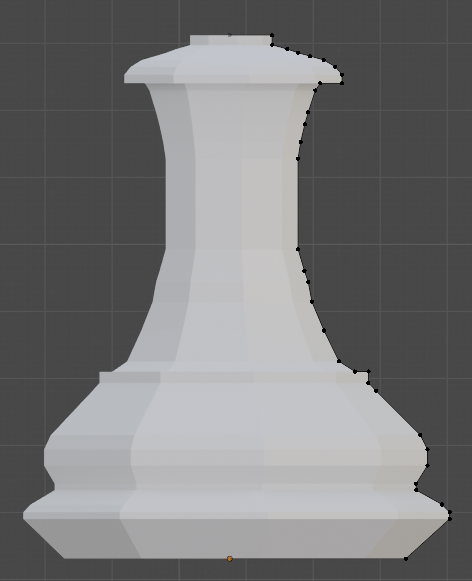
\includegraphics[height=150pt]{Images/pawn model.png}
\end{center}
The notable changes from the default settings is the lowering of the steps from
\(16 \to 10\) and disabling \texttt{Smooth Shading}. This was a stylistic choice as it
was believed that the low polygon look would better demonstration reflections and
the planned indirect lighting (See \hyperref[sec:org3e00aea]{Lighting - Disco Ball}).

To model the knight, 3 separate reference images where used. The base was
constructed in a similar manner to the other pieces. The head was modelled
manually (read painstakingly).

\begin{figure}[htbp]
\begin{center}
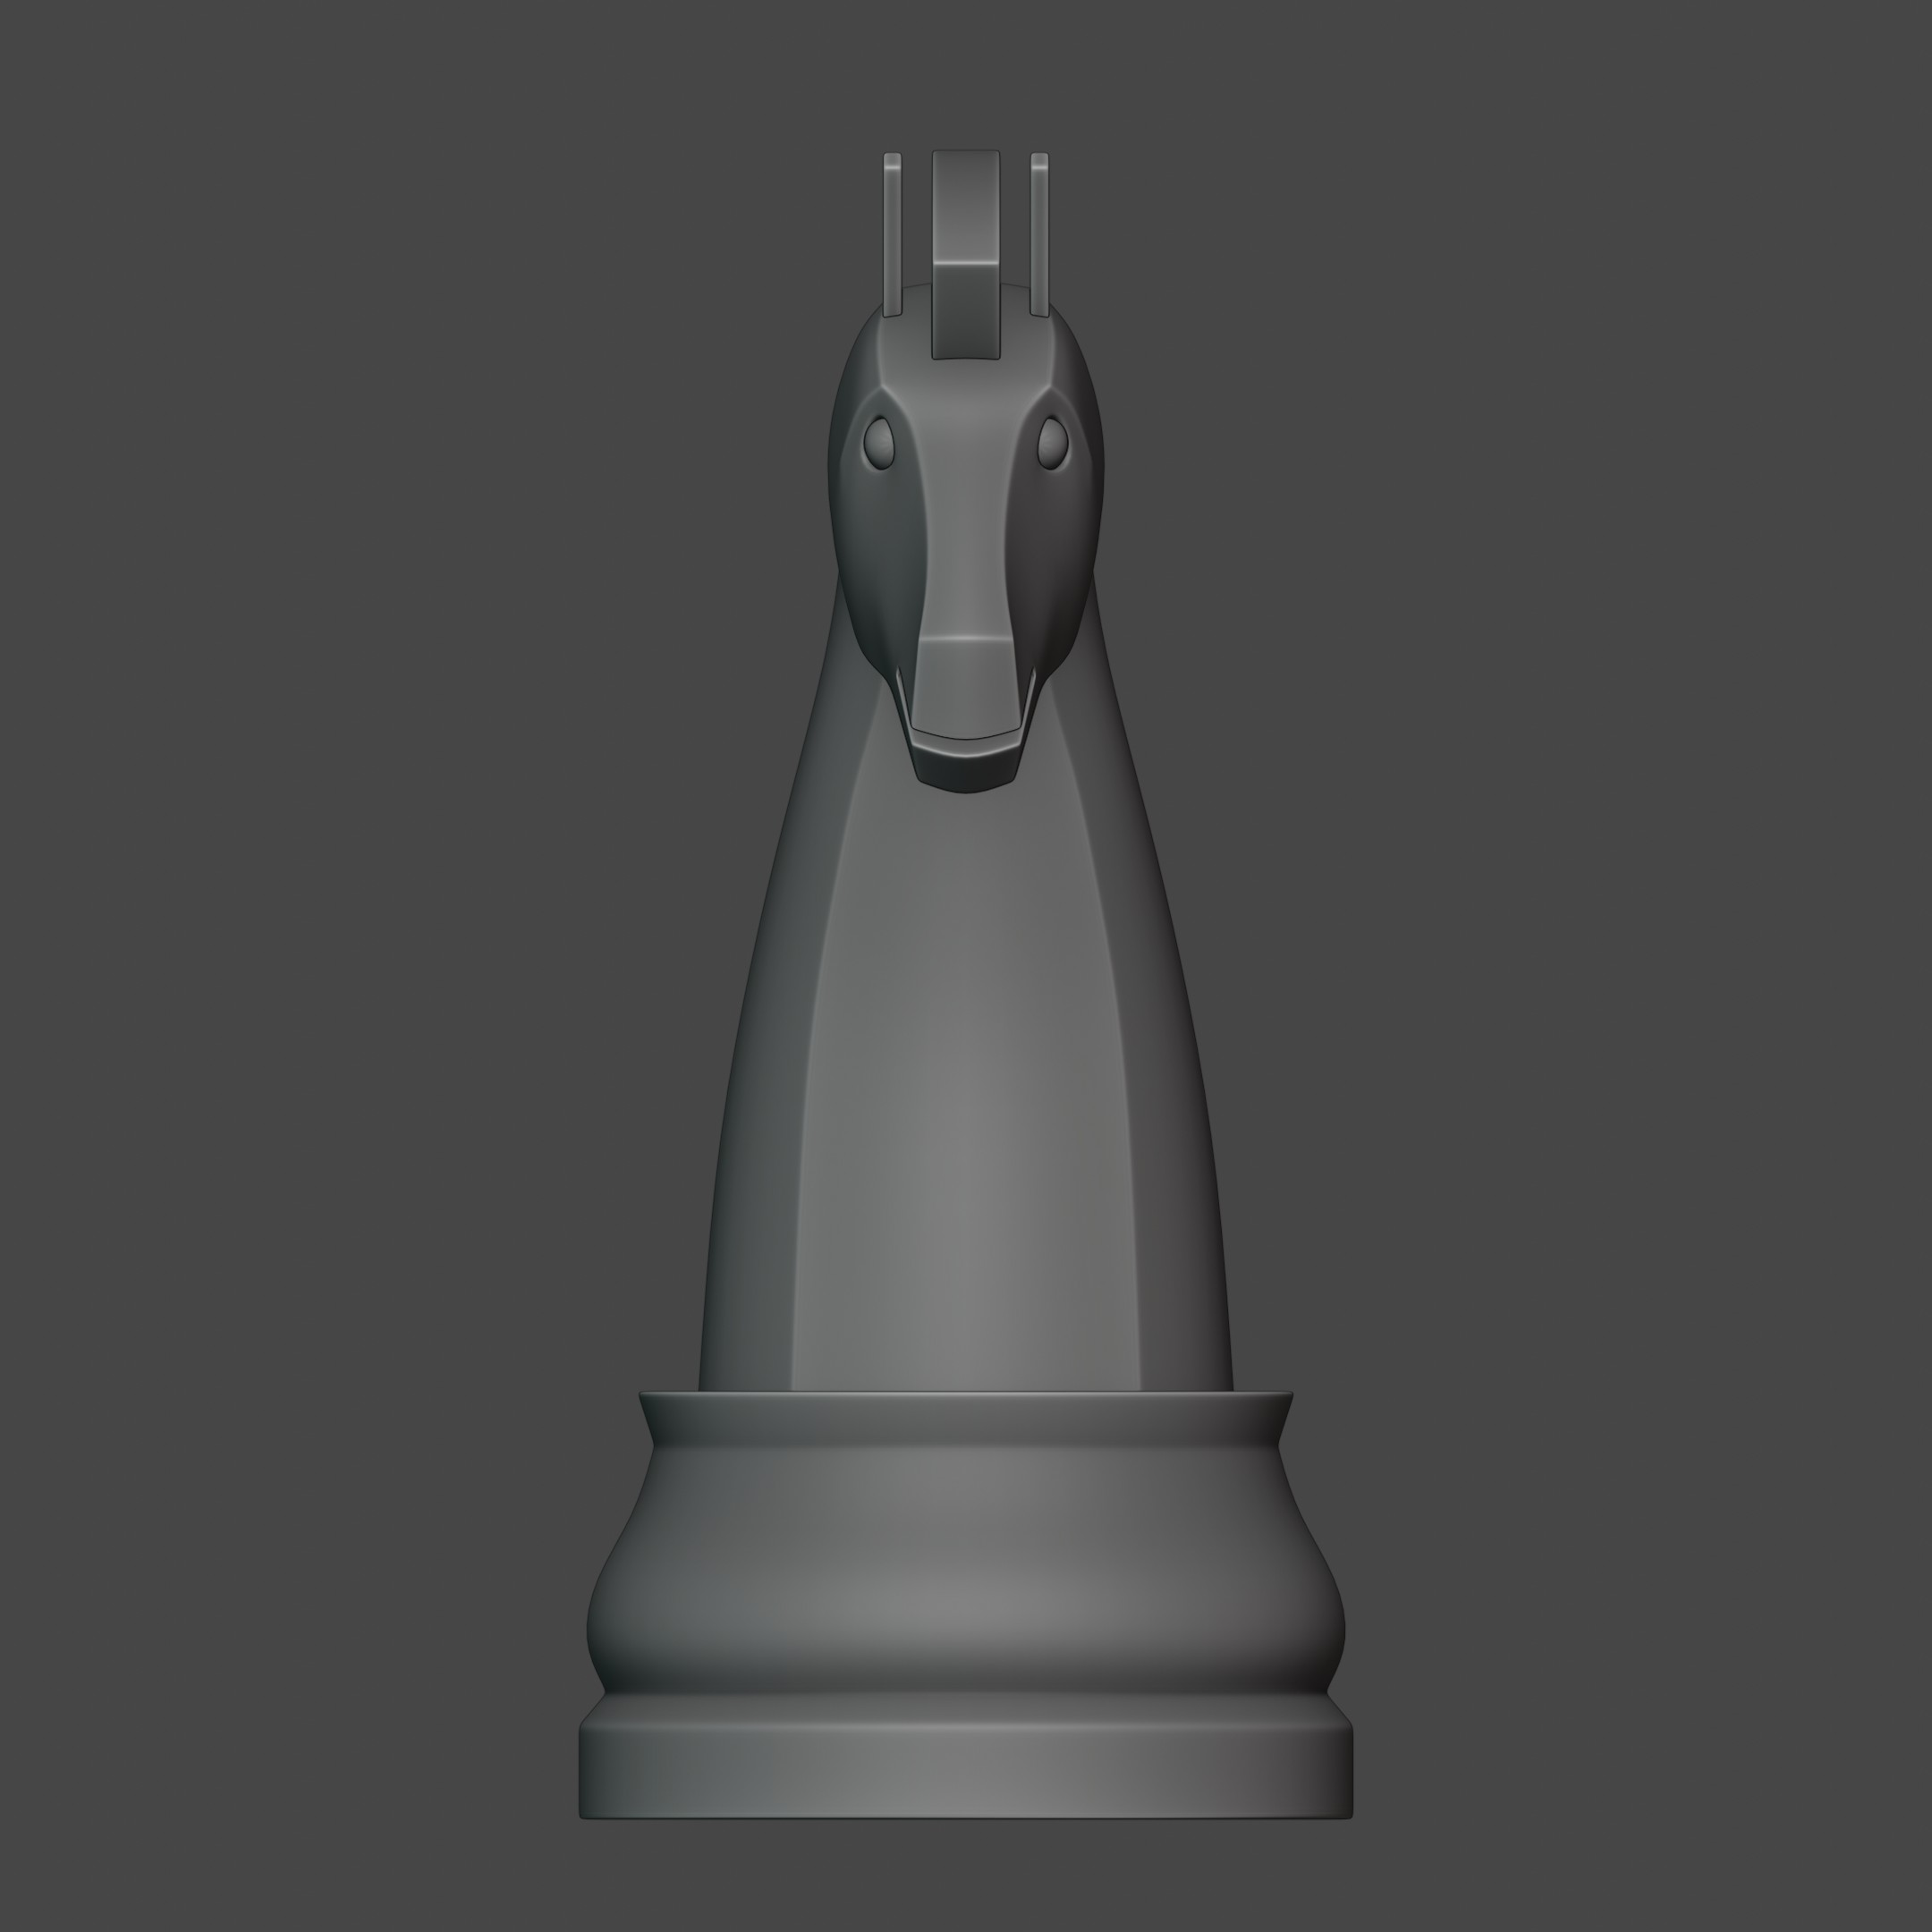
\includegraphics[width=0.3\textwidth]{ref/knight front.jpg}

\includegraphics[width=0.3\textwidth]{ref/knight right.jpg}
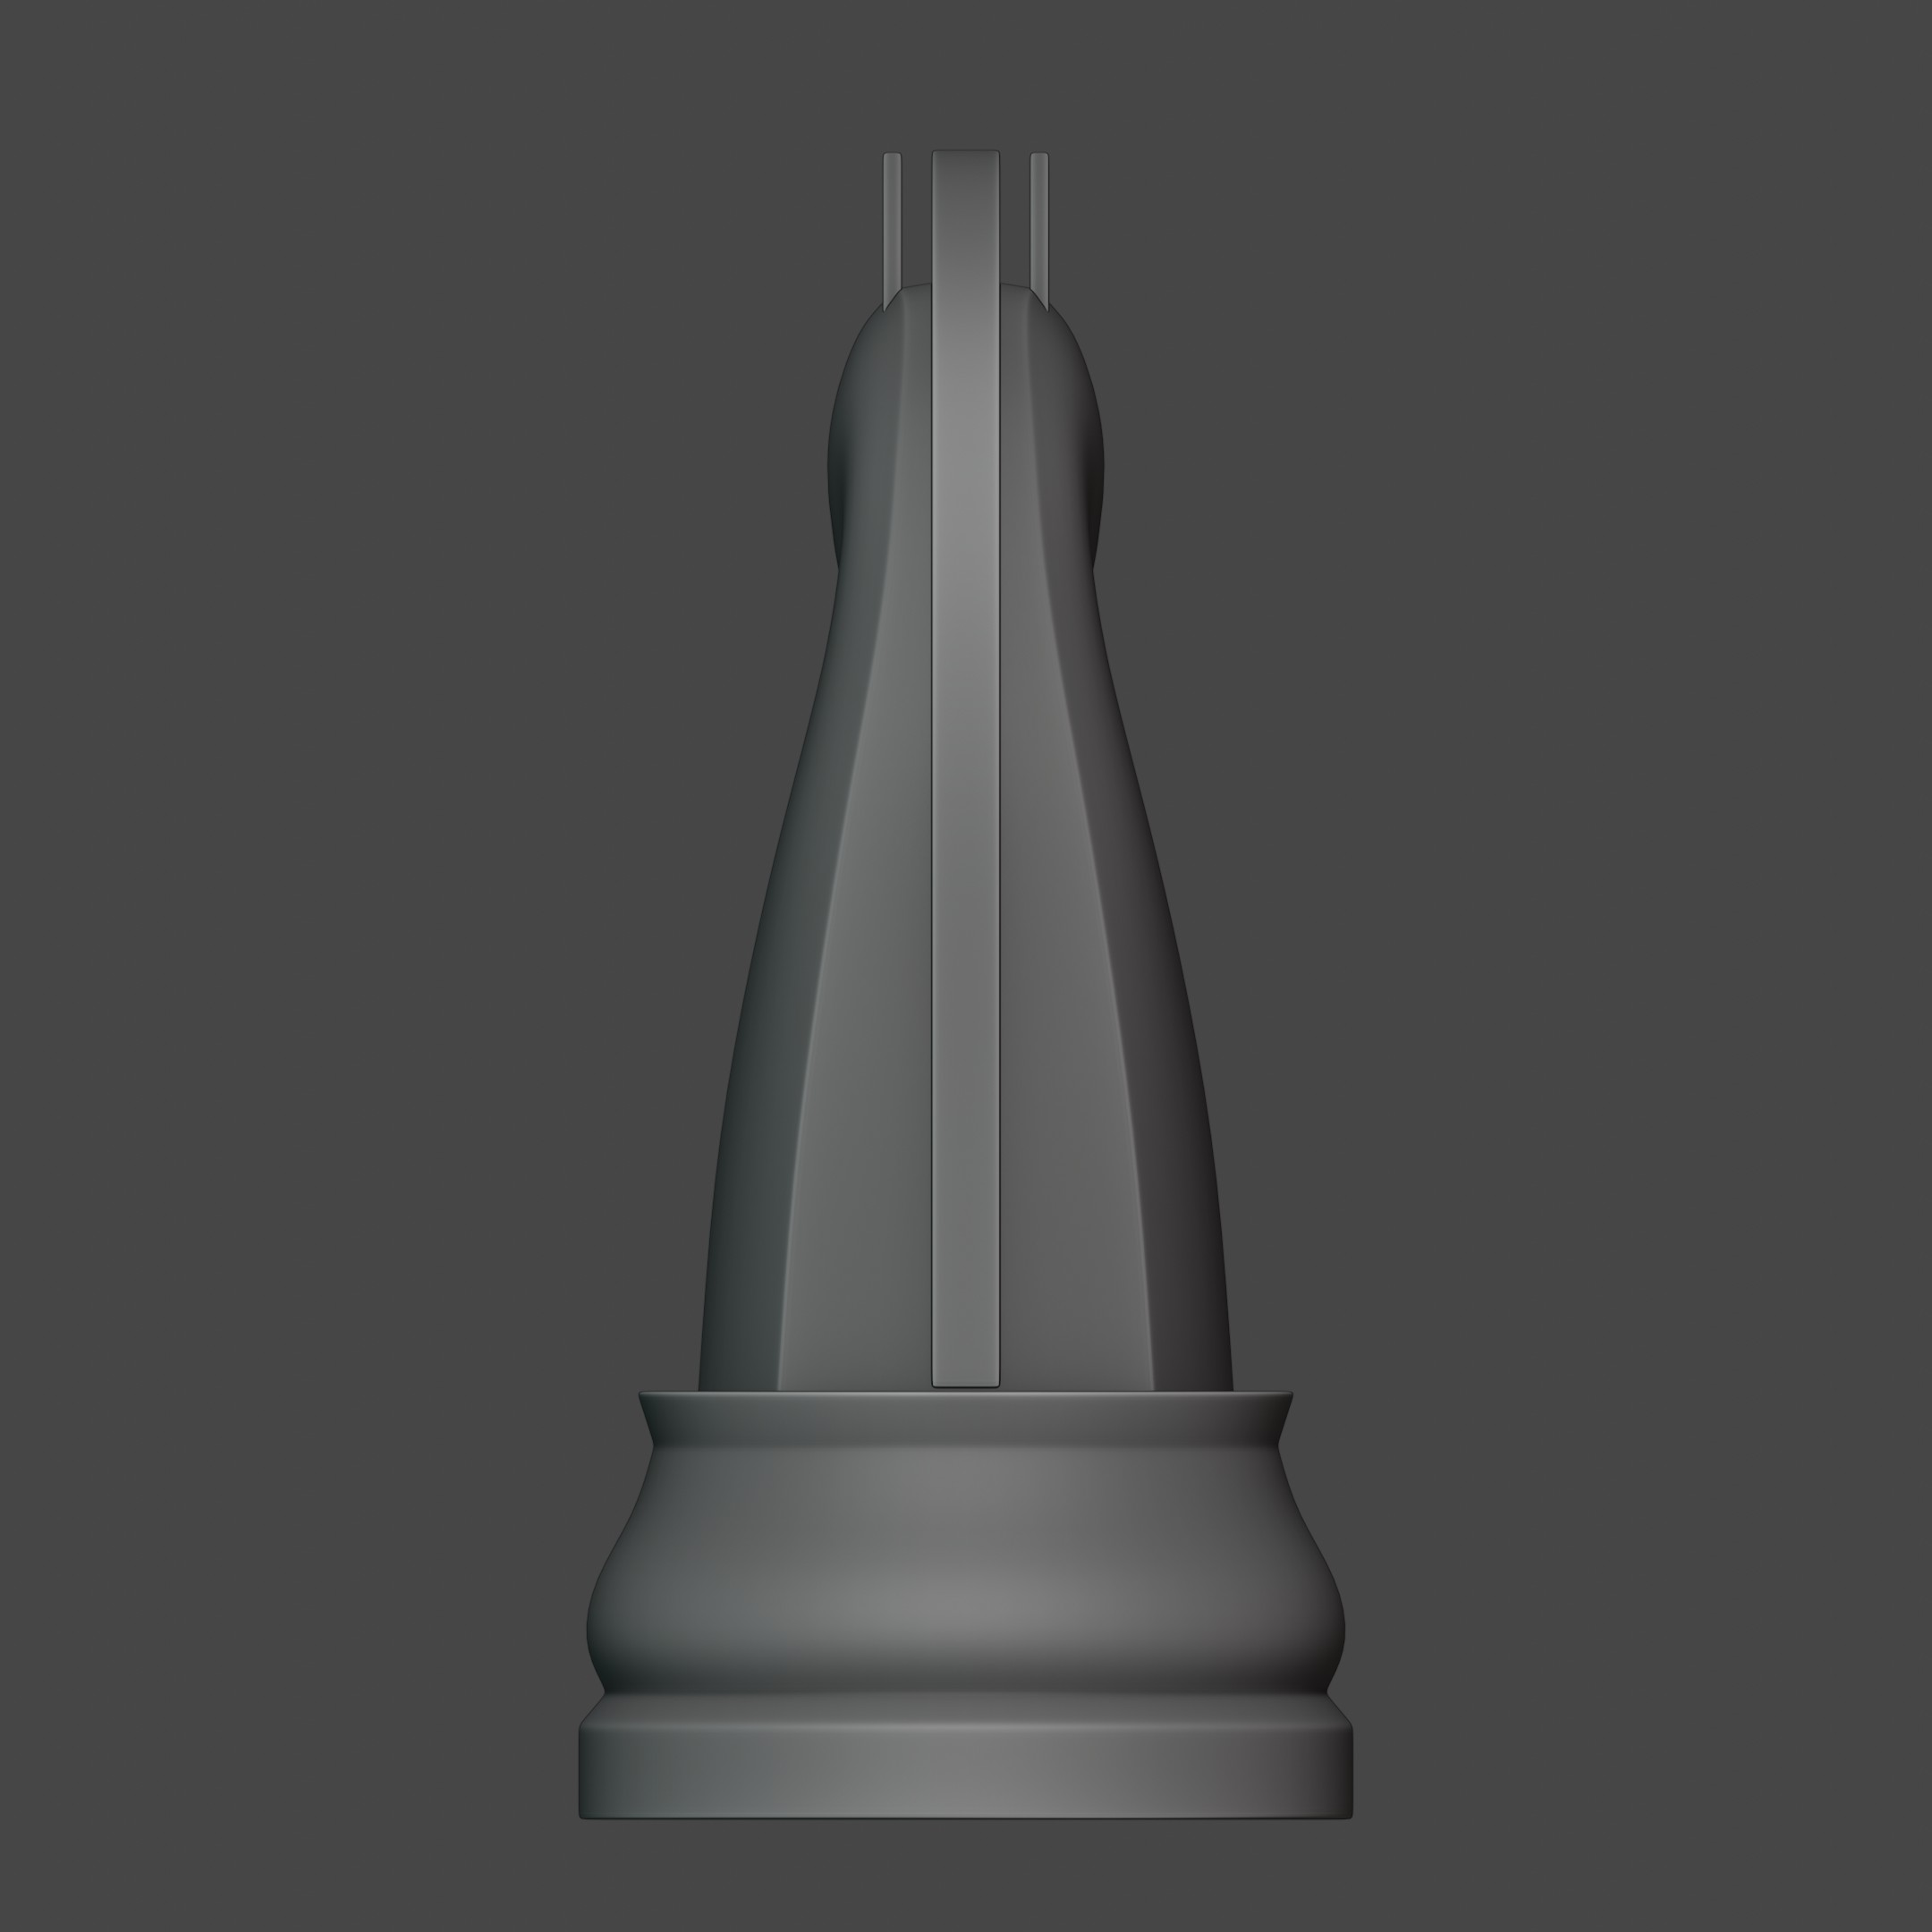
\includegraphics[width=0.3\textwidth]{ref/knight back.jpg}
\end{center}
\caption{Knight reference images, \href{https://imgur.com/a/Pg9WYII}{(Source)}}
\end{figure}

Additionally ico-spheres where added  to piece some pieces additional detail.
The finally piece models appear as below.
\begin{center}
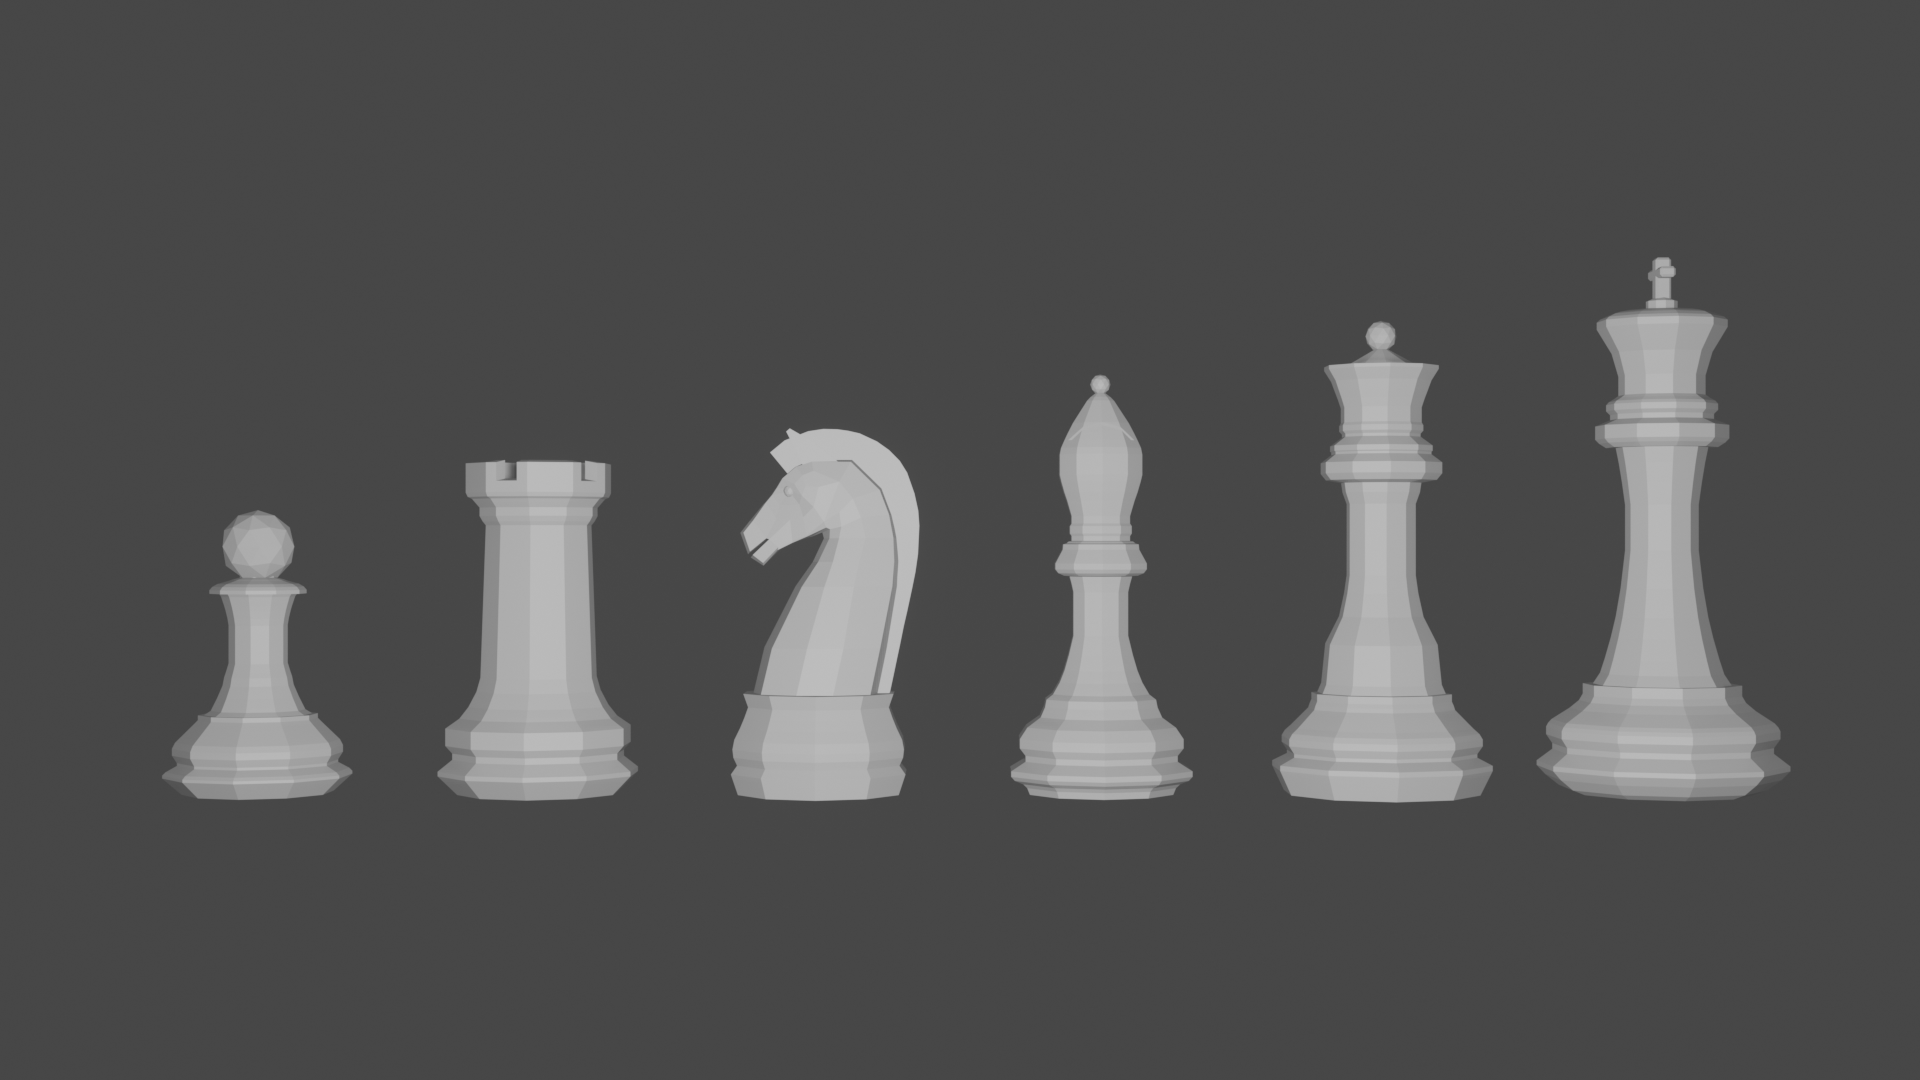
\includegraphics[width=0.5\textwidth]{Images/Pieces.png}
\end{center}
\subsubsection{Board}
\label{sec:org6201923}
\paragraph{Chess board}
\label{sec:orgba182e4}
The chess board model is a simple rectangular based prism with dimensions \texttt{8m x
8m x 0.4m}. The checker board texture comes from the \texttt{Checker Texture}, with
\texttt{scale=8.0} and black and white colours. This texture output is then feed into
the base colour input of a \texttt{Principled BSDF} shader node.

\begin{figure}[htbp]
\centering
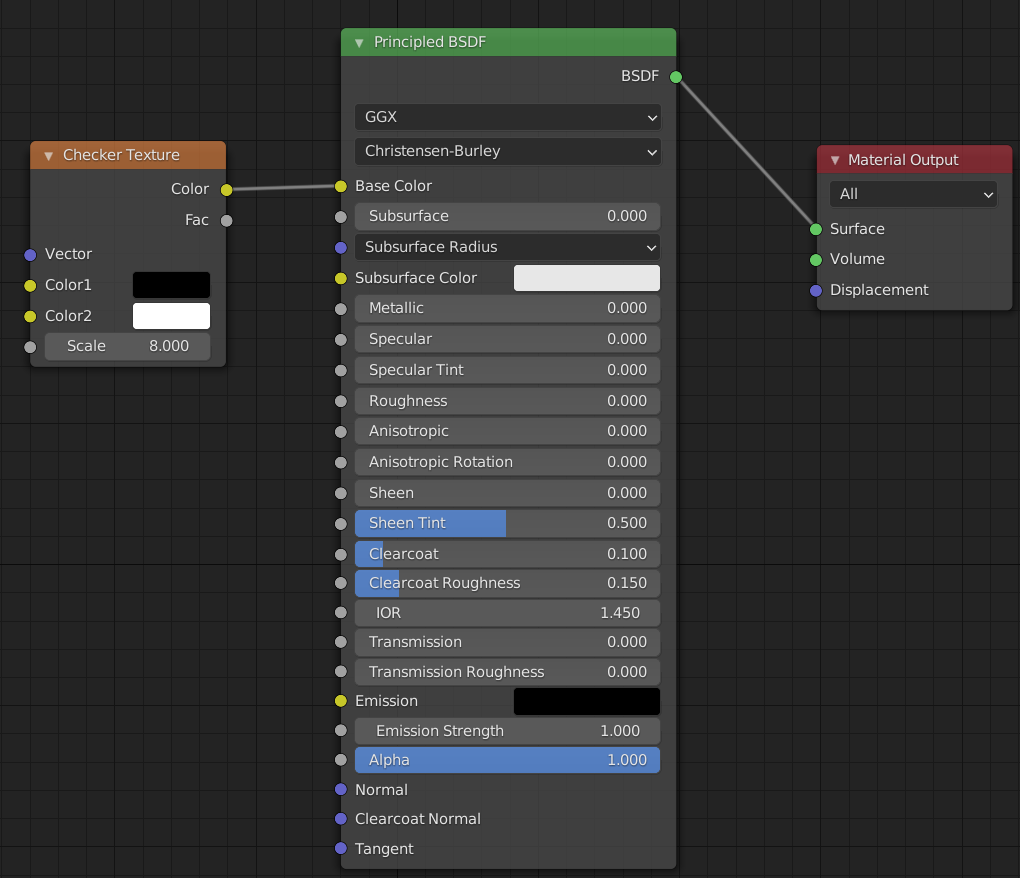
\includegraphics[width=350pt]{Images/checker texture.png}
\caption{\label{checker-texture}Complete checker board texture.}
\end{figure}

Within world space the board was positioned in the positive, positive quadrant
such that the very bottom left handle corner of the board was at \texttt{0,0}
with each squares dimensions as \texttt{1m x 1mx}. This positioning becomes important
in \hyperref[sec:org789c6c4]{Python implementation - Array index to world space}.
\paragraph{Marble exterior}
\label{sec:org973e6ac}
\subsection{Particle effects}
\label{sec:orgfe36209}
\subsubsection{Explosions}
\label{sec:orgac09548}
Initially an explosion was planned an each piece capture as a way to add some
flare. However this was quickly scrapped as the baking and rendering time costs
were deemed obscene. A demo render was created and can be viewed here TODO FIX
THIS
\subsubsection{Confetti}
\label{sec:orga7f18d5}
As an alternative to explosions, a confetti shower on the winning king (only
checkmates deserve confetti) was added instead.

The confetti is still an explosion, however the outgoing particles are set to a
collection of ``confetties''. The source of the explosion is a upwards facing
dome, this gives the confetti a nice even spread. The particles are set to have
randomised, size, rotation, angular velocity, normal velocity. To achieve the
slow fall effect the effective gravity of the particle simulation was lowered to
38\% its normal strength. Each confetti has a texture with \texttt{Roughness 1.0} and
varying base colours.

\begin{figure}[htbp]
\begin{center}
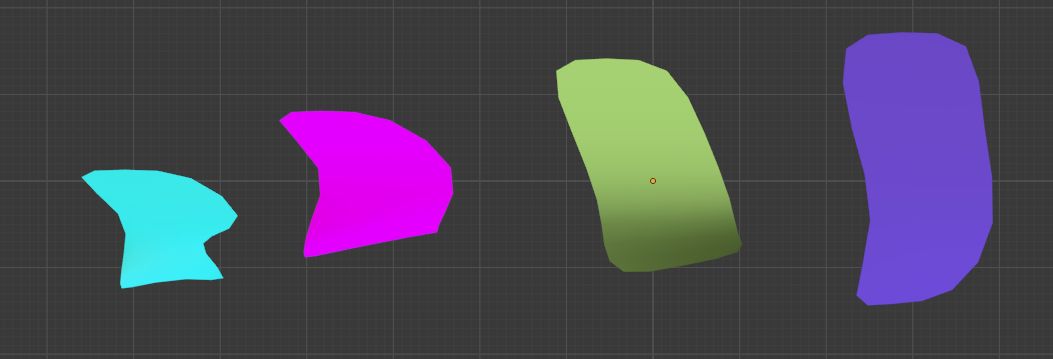
\includegraphics[width=0.5\textwidth]{Images/confetties.png}
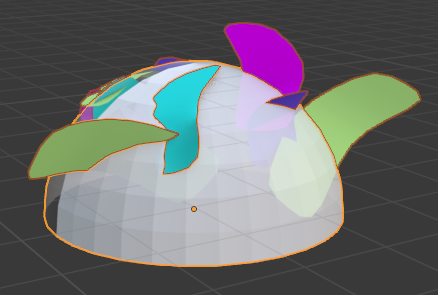
\includegraphics[width=0.3\textwidth]{Images/confetti dome.png}
\end{center}
\caption{Confetties (left), confetti source (right)}
\end{figure}

A sample render can be seen below.
\begin{figure}[htbp]
\centering
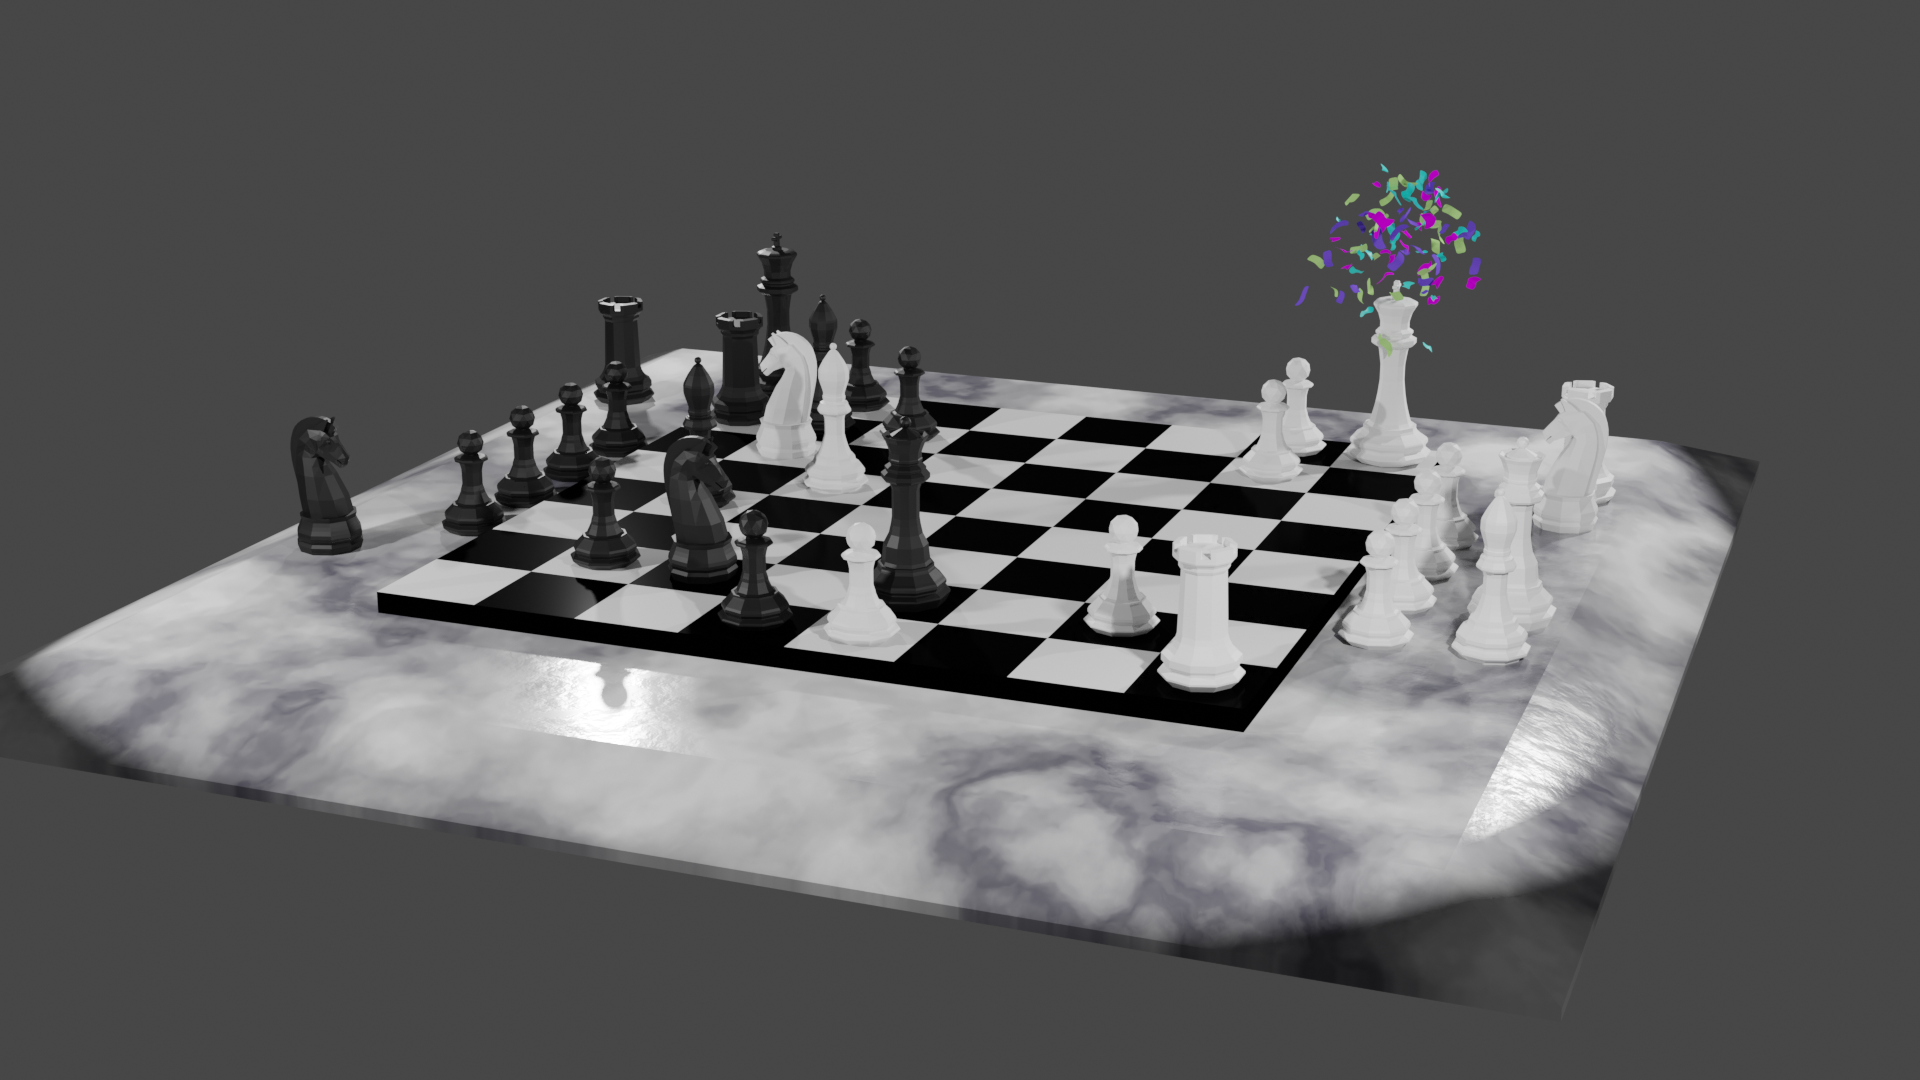
\includegraphics[width=\textwidth]{Images/Confetti! cycles.png}
\caption{Confetti render using Cycles}
\end{figure}
\subsection{Lighting}
\label{sec:org6468a44}
\subsubsection{Direct}
\label{sec:orgbba6fbd}
\subsubsection{Indirect}
\label{sec:org190985b}
\subsubsection{Disco ball}
\label{sec:org3e00aea}
\subsection{Render engine}
\label{sec:orgf5baf58}
\subsubsection{Eevee}
\label{sec:org57300c3}
\subsubsection{Cycles}
\label{sec:orgbe5d7ea}
\paragraph{Thank you to Jack}
\label{sec:orga6da89f}
Due to significant hardware limitations for ray-tracing (\texttt{GTX 760, i5-4670}), a
favour was called in with a good friend, Jack kindly lent their \texttt{RTX 2070}  for a
cycles render. See \href{https://github.com/Jake-Moss/blender-chess/blob/master/Videos/Marble\_cycles.mp4}{master/Videos/Marble\_cycles.mp4}.
\subsubsection{Luxcore}
\label{sec:org2bf891a}
\subsubsection{Tragedy - 22:20, 01/June/2021}
\label{sec:org18a09d9}
At 10:20pm on the first of June the PC that had been enslaved to rendering a
Luxcore for more than 96 hours straight, died. It had been a good 8 years, but
she finally gave out. Official cause of death is unknown but it suspected to be
something to do with power delivery.

A successful data recovery was conducted the next morning. Only the last 12
frames were missing, they were rendered on another device. See
\href{https://github.com/Jake-Moss/blender-chess/blob/master/Videos/disco\_luxcore.mp4}{master/Videos/disco\_luxcore.mp4 }
\section{Python implementation}
\label{sec:orgd46f993}
\subsection{Processing games}
\label{sec:org8e86f52}
Reading and stepping through games is handled almost entirely by the chess
library. No special considerations need to be made here. The minium working
example below demonstrates all that is necessary to step through an entire game.

\begin{Code}
\begin{Verbatim}[]
\color[HTML]{383a42}\EFk{import} chess
\EFk{with} \EFb{open}(filename) \EFk{as} \EFv{pgn}:
    game = chess.pgn.read\_game(pgn) \EFcd{\# }\EFct{Parses pgn file}
    \EFv{board} = game.board()

    \EFk{for} move \EFk{in} game.mainline\_moves():
        board.push(move) \EFcd{\# }\EFct{Pushs the move to the move stack, this "makes" the move}
\end{Verbatim}
\end{Code}
\subsection{Pairing problem}
\label{sec:orgc1a7183}
During a game of chess there is nothing in between moves, simply one discrete
board state after another. This is also how the chess library makes moves, by
computing differences and tracking board states, while this is reliable and
simple it does not play nice when games become continuous (animated).

Initially this script also tracked the board state using a dictionary, with the
square as the key, and corresponding blender object as the value, pushing and
pop at each move. However, this presented difficulties when implementing
animations and special moves and animations. The code was generally cluttered
and not up to an acceptable quality.
\subsection{The solution}
\label{sec:orgc7287a9}
To remedy the mentioned problems a custom class was devised, and aptly name
\texttt{CustomPiece}. This class acts as a generalised representation of a piece which
is able to act upon itself and the Blender model it puppets. Stored within an
unrolled 2d array with the index representing its position on the chess board
(See \hyperref[sec:org789c6c4]{Python implementation - Array Index to world space}) the object is able to
move itself within the array while handling move and capture animations. Special
move handling is generalised into the main loop, (See \hyperref[sec:orgc8b627b]{Python implementation -
Special moves}).

This design approach has clear advantages such as
\begin{itemize}
\item Adheres to the \texttt{Model-View-Controller} design philosophy.
\item Array and object manipulation is not handled at any higher level than required.
\item Translation between the chess library interface and Blenders API is seamless.
\item Creates a unique object that pairs a Blender model to a \texttt{python-chess}
\texttt{PieceType}.
\end{itemize}
However, the self-referential nature of objects manipulating the array their
are stored in adds significantly to the complexity. Luckily the implementation is
simple.

An initial sketch of this class can be seen here \ref{class-sketch}.

Implementation can be see here \ref{class-src}.
\subsection{Array index to world space}
\label{sec:org789c6c4}
\texttt{python-chess} provides great functionality to retrieve what square a move is
coming from, and going to. Internally this is stored as a \texttt{int} representing
each square in 1d array notation.

\begin{minipage}{0.5\textwidth}
\begin{Code}
\begin{Verbatim}[]
\color[HTML]{383a42}\EFv{Square} = \EFb{int}
\EFv{SQUARES} = [
    A1, B1, C1, D1, E1, F1, G1, H1,
    A2, B2, C2, D2, E2, F2, G2, H2,
    A3, B3, C3, D3, E3, F3, G3, H3,
    A4, B4, C4, D4, E4, F4, G4, H4,
    A5, B5, C5, D5, E5, F5, G5, H5,
    A6, B6, C6, D6, E6, F6, G6, H6,
    A7, B7, C7, D7, E7, F7, G7, H7,
    A8, B8, C8, D8, E8, F8, G8, H8,
] = \EFb{range}(\EFhn{64})
\end{Verbatim}
\end{Code}
\end{minipage}
\begin{minipage}{0.5\textwidth}
\setchessboard{color=black,clearboard,showmover=false}
\chessboard[
pgfstyle=
{[base,at={\pgfpoint{0pt}{-0.3ex}}]text},
text= \fontsize{1.2ex}{1.2ex}\bfseries
\sffamily\getfieldnumber\currentwq,
markboard]
\end{minipage}
\newpage
\begin{figure}[htbp]
\centering
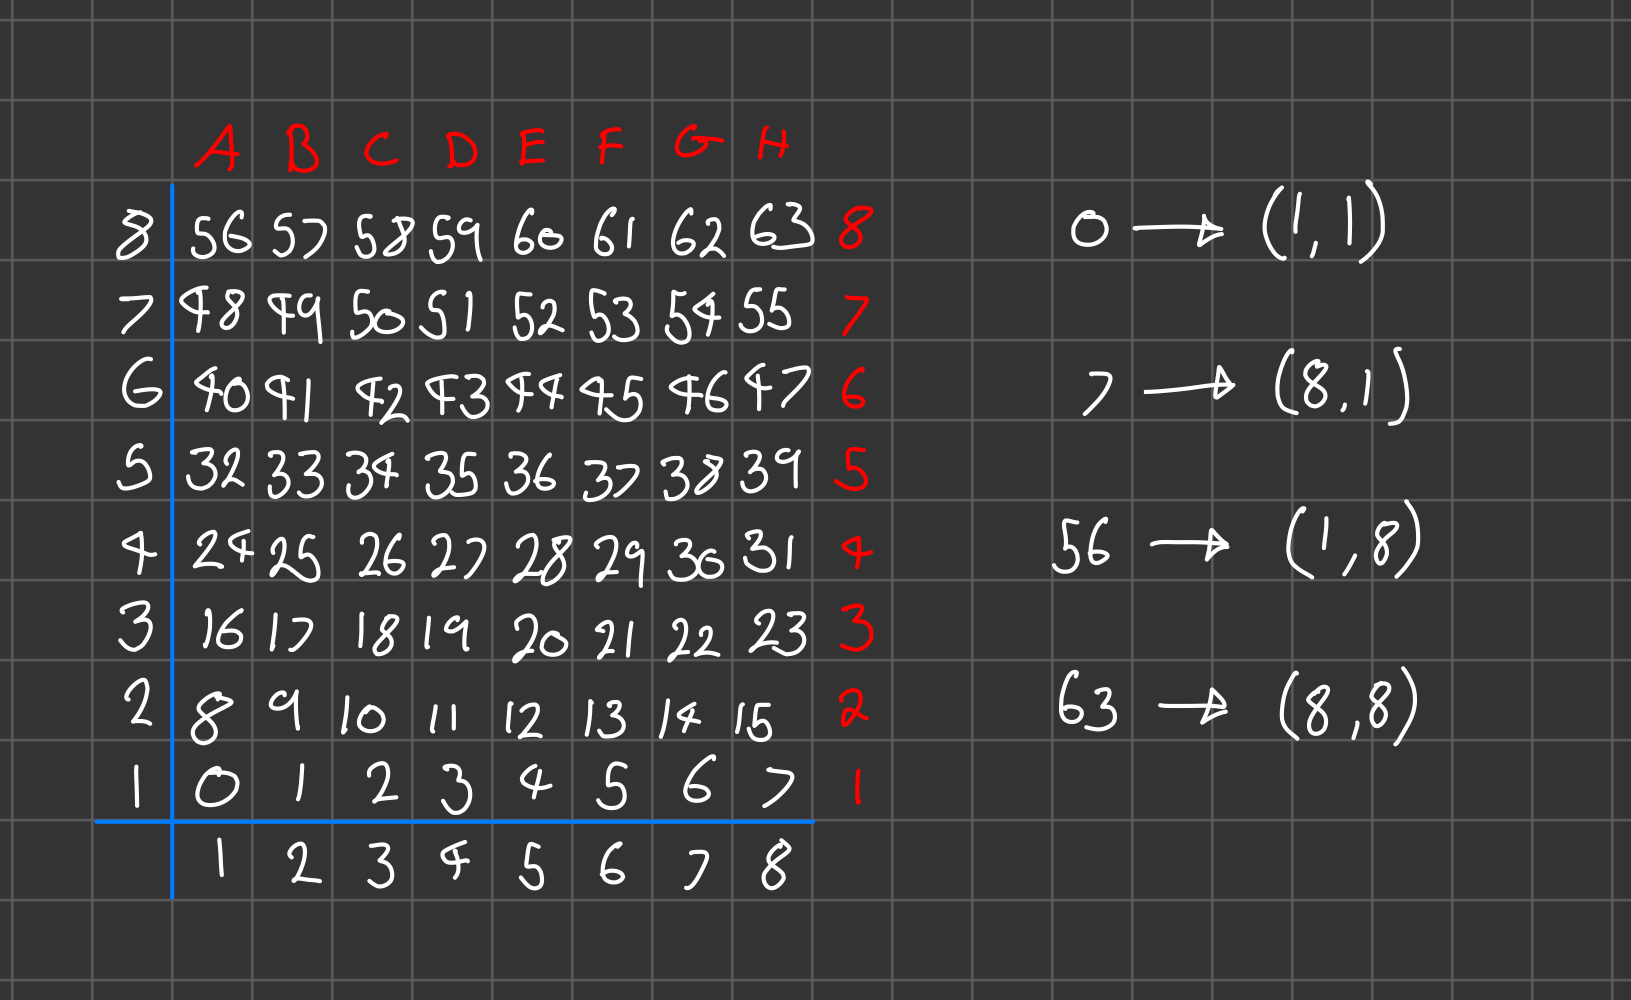
\includegraphics[width=0.5\textwidth]{Images/array.png}
\caption{\label{array-working}Array representation ((\texttt{tl}) Source code, (\texttt{tr}) Chess board, (\texttt{b}) Overlaid)}
\end{figure}

To convert form array indexing two simple expressions were used.
\[x = (\text{INDEX mod } 8) + 0.5\]
\[y = (\text{INDEX div } 8) + 0.5\]\footnote{Note \texttt{div} here is integer division.}
Note the addition of \(0.5\) is to centre the pieces on the board squares in
world space and will be excluded from further examples.
\subsubsection{Abuse of this functionality}
\label{sec:org6bf530f}
\begin{wrapfigure}[14]{r}{0.4\textwidth}
\centering
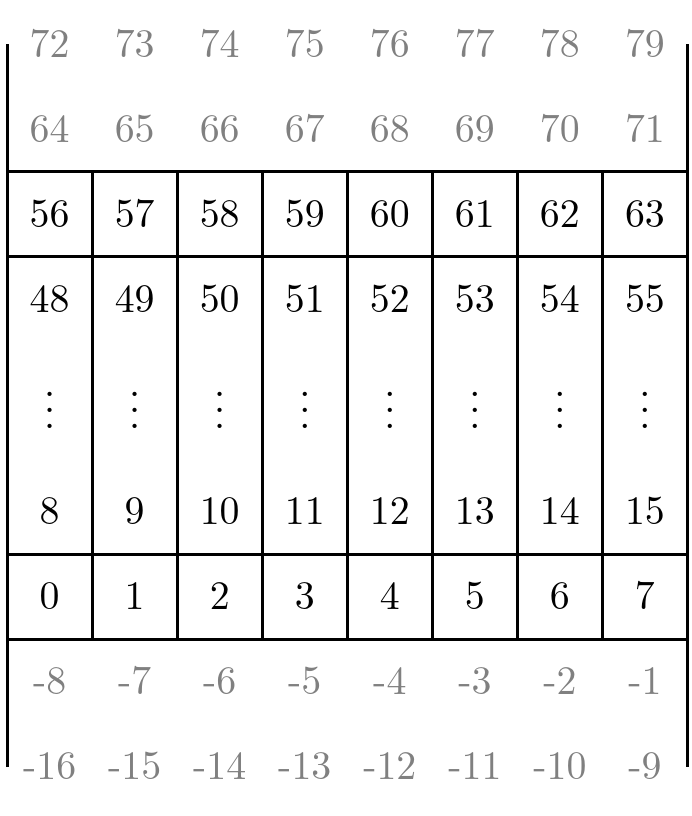
\includegraphics[width=0.35\textwidth]{Images/tikzit_image0.png}
\caption{\label{extended-array}Extended conversion}
\end{wrapfigure}

While modulo will always produce a positive integer between \(0 \to 7\), integer
division can result negative numbers and is not bounded. Using this the mapping
can be extended past the board it was designed for.

This provides an easy method to place captured piece after their animation. By
storing each pieces initial position, and adding or subtracting \(16\) depending on
the colour, pieces can be placed \(2\) rows behind their initial position.

Two rows behind was preferable to the respective position on the other side of
the board to avoid the inversion required so that the pawns would be in front of the
back rank pieces.

\newpage
\subsection{Special moves}
\label{sec:orgc8b627b}
Figure \ref{flowchart} shows the main loop logic, used to move the correct pieces.
\begin{figure}[htbp]
\centering
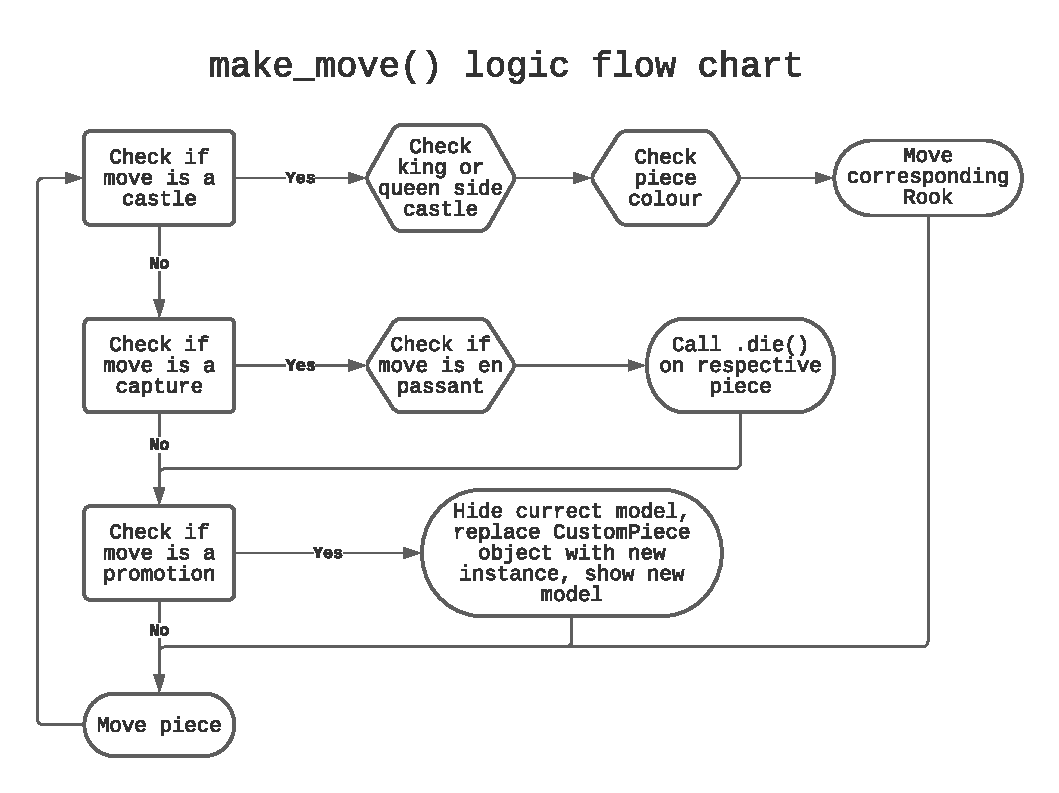
\includegraphics[width=\textwidth]{flowchart.pdf}
\caption{\label{flowchart}Main loop logic}
\end{figure}
\subsubsection{Castling}
\label{sec:org0256cff}
Within standard chess there are only four castling possibilities, these are easy
enough to check naively. This is the only section that limits this script to
standard chess. To extend support to \texttt{chess960}, a bit-board mask of all the
rooks with castling rights could be filtered to obtain the index of the rook
that will be castled. See \href{https://python-chess.readthedocs.io/en/latest/core.html?highlight=castl\#chess.Board.castling\_rights}{the documentation.}
\begin{Code}
\begin{Verbatim}[]
\color[HTML]{383a42}\EFk{if} board.is\_castling(move):
    \EFk{if} board.turn: \EFcd{\# }\EFct{White}
        \EFk{if} board.is\_kingside\_castling(move):
            array[chess.H1].move(chess.F1)
        \EFk{else}: \EFcd{\# }\EFct{queen side}
            array[chess.A1].move(chess.D1)
    \EFk{else}: \EFcd{\# }\EFct{Black}
        \EFk{if} board.is\_kingside\_castling(move):
            array[chess.H8].move(chess.F8)
        \EFk{else}: \EFcd{\# }\EFct{queen side}
            array[chess.A8].move(chess.D8)
\end{Verbatim}
\end{Code}
\subsubsection{En passant}
\label{sec:orga864584}
The \texttt{python-chess} library makes handling en passant a breeze. The move is
checked if it is an en passant first, then as only one square is possible of an
en passant on any move that position is retrieved.
\begin{Code}
\begin{Verbatim}[]
\color[HTML]{383a42}    \EFk{else}: \EFcd{\# }\EFct{standard case}
        \EFk{if} board.is\_capture(move):\EFcd{\# }\EFct{is en passant, great...}
            \EFk{if} board.is\_en\_passant(move):
                array[board.ep\_square].die() \EFcd{\# }\textcolor[HTML]{c3e88d}{\textbf{NOTE}}\EFct{, object is gc'ed}
            \EFk{else}: \EFcd{\# }\EFct{its a normal capture}
                array[locTo].die() \EFcd{\# }\textcolor[HTML]{c3e88d}{\textbf{NOTE}}\EFct{, object is gc'ed}
\end{Verbatim}
\end{Code}
\subsubsection{Promotion}
\label{sec:org69e6695}
Contained within a separate conditional is the promotion logic. This is handled
separately from the rest of the logic as a move can be both a capture and a
promotion.
\begin{Code}
\begin{Verbatim}[]
\color[HTML]{383a42}    array[locFrom].move(locTo) \EFcd{\# }\textcolor[HTML]{c3e88d}{\textbf{NOTE}}\EFct{, piece moves always}

    \EFk{if} move.promotion \EFk{is} \EFk{not} \EFc{None}:
        array[locTo].keyframe\_insert(data\_path=\EFs{"location"}, index=-\EFhn{1})
        array[locTo].hide\_now() \EFcd{\# }\EFct{hide\_now unlinks within blender}
        pieceType = move.promotion \EFcd{\# }\EFct{piece type promoting to}
        array[\EFv{locTo}] = CustomPiece(chess.Piece(pieceType, board.turn),\char92{}
                                   SOURCE\_PIECES[chess.piece\_symbol(pieceType)],\char92{}
                                   array, locTo) \EFcd{\# }\EFct{shiny new object}
        array[locTo].show\_now()
\end{Verbatim}
\end{Code}
A new key-frame is inserted initially as the piece that will promote has already
been moved and that animation needs to finish before it can be hidden.

Within the Blender view port the pieces that will be promoted too already exist
at the right position, they are just not rendered until needed.
\subsection{Animation}
\label{sec:orgbb0100e}
\subsubsection{Key frames}
\label{sec:org4c34590}
To animate an object within blender two key-frames must be inserted with
different values for some property at varying times. Blender will then
interpolate between them (See \hyperref[sec:org3e8ac5b]{Python implementation - Interpolation} for
interpolation methods)

Key-frames for all pieces are inserted every move. This is done to ensure
stationary pieces stay stationary. Every move the piece has \(10\) frames to
complete its moving animation. Between each move there a \(3\) buffer to provide
some separation between moves.

In addition to piece animations, the camera also rotates at a rate of
\(2^{\circ}\) per \(13\) frames.
\begin{Code}
\begin{Verbatim}[]
\color[HTML]{383a42}        \EFv{FRAME\_COUNT} = \EFhn{0}
        keyframes(array) \EFcd{\# }\EFct{intial pos}
        \EFv{FRAME\_COUNT} += \EFhn{10}
        \EFk{for} move \EFk{in} game.mainline\_moves():
            scene.frame\_set(FRAME\_COUNT)

            make\_move(board, move, array)
            keyframes(array) \EFcd{\# }\EFct{update blender}

            camera\_parent.\EFv{rotation\_euler}[\EFhn{2}] += radians(\EFhn{2}) \EFcd{\#}\EFct{XYZ}
            camera\_parent.keyframe\_insert(data\_path=\EFs{"rotation\_euler"}, index=-\EFhn{1})

            board.push(move) \EFcd{\# }\EFct{update python-chess}

            FRAME\_COUNT += \EFhn{10}
            keyframes(array) \EFcd{\# }\EFct{update blender}
            FRAME\_COUNT += \EFhn{3}
\end{Verbatim}
\end{Code}

While the camera's rotation is tired to the length of the game, in order to
continue spinning while the remaining animations (confetti and captures) finish additional key frames
are added. Confetti is conditionally added to the winning king. No confetti for a draw.
\begin{Code}
\begin{Verbatim}[]
\color[HTML]{383a42}        \EFv{confetti} = bpy.data.collections[\EFs{"Board"}].objects[\EFs{'Confetti source'}]
        \EFk{if} board.outcome() \EFk{is} \EFk{not} \EFc{None}:
            winner = board.outcome().winner
            \EFv{king\_square} = board.king(winner)
            \EFv{xTo}, \EFv{yTo} = square\_to\_world\_space(king\_square)
            confetti.\EFv{location} = Vector((xTo, yTo, \EFhn{3}))
            bpy.data.particles[\EFs{"Confetti"}].\EFv{frame\_start} = FRAME\_COUNT
            bpy.data.particles[\EFs{"Confetti"}].\EFv{frame\_end} = FRAME\_COUNT + \EFhn{12}

        \EFk{print}(FRAME\_COUNT)
        \EFk{for} \_ \EFk{in} \EFb{range}(\EFhn{5}):
            scene.frame\_set(FRAME\_COUNT)
            camera\_parent.\EFv{rotation\_euler}[\EFhn{2}] += radians(\EFhn{2}) \EFcd{\#}\EFct{XYZ}
            camera\_parent.keyframe\_insert(data\_path=\EFs{"rotation\_euler"}, index=-\EFhn{1})

            FRAME\_COUNT += \EFhn{13}
\end{Verbatim}
\end{Code}
In order to move the camera with a fixed rotation and radius from the centre of
the board the camera was made a child of a \texttt{Empty Plain Axis}. Rotations and
translations applied to the camera parent are also applied to the camera. This
allows for ease fixed distance rotations.
\begin{figure}[htbp]
\centering
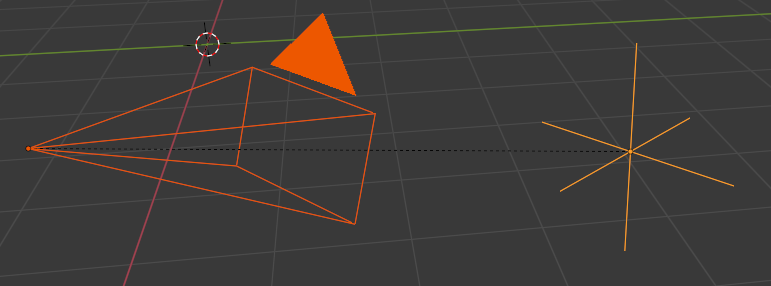
\includegraphics[width=0.5\textwidth]{Images/camera parent.png}
\caption{\label{camera-parent}Camera parent axis}
\end{figure}
\subsubsection{Interpolation}
\label{sec:org3e8ac5b}
Blender offers 3 curves for interpolation between key-frames.
\begin{itemize}
\item Constant\\
Object value only objects on the last possible frame.
\item Linear\\
Object value has a changes linear between the key-frames to form piecewise
continuous curve.
\item Bézier\\
The object value is interpolated using a Bézier curve. Bézier curves are
parametric curves used in computer graphics to create smooth surfaces, or in
this case, a smooth function between two points.

Blender implements a forward differencing method for a cubic Bézier curve
evident from the source code \cite{blender-source}.
\end{itemize}
By default Blender uses Bézier curve interpolation for all motions. This is the
preferred option for piece movement. However, linear was opted for the camera
motion although a cubic Bézier curve would produce the same outcome as it made
debugging slightly easier.
\subsection{Reproducibility}
\label{sec:org5a3ca3e}
This project was created used
\begin{itemize}
\item Blender \texttt{2.92}
\url{https://www.blender.org/}
\item Python \texttt{3.9.5} \footnote{Blender comes bundled with this version. If the system python is used
instead ensure it matches the version Blender was built with and is above \texttt{3.7}
for the \texttt{\_\_future\_\_} module. Past \texttt{3.10} the \texttt{\_\_future\_\_} module is no longer required.}
\url{https://www.python.org/}
\item python-chess \texttt{1.5.0} \footnote{This project requires the \texttt{Outcome} class released in \texttt{1.5.0}}
\url{https://github.com/niklasf/python-chess}
\end{itemize}
\subsubsection{Python environment}
\label{sec:orgd1e9c32}
Blender is distributed with its own python installation for consistency, however
this means that installed python modules are not present
\cite{blender-python-env}. To mitigate this the \texttt{-{}-target} flag for \texttt{pip install}
can be used to install directly to the blender python environment
\cite{pip-install-man}.
\begin{Code}
\begin{Verbatim}[]
\color[HTML]{383a42}pip install -t \char126{}/.config/blender/2.92/scripts/modules chess
\end{Verbatim}
\end{Code}
This ensures Blenders \texttt{Python} will has access to the required libraries for this
script to function.

\section{Results}
\label{sec:org14d00d0}
\section{Evaluation}
\label{sec:org8bd6252}

\newpage
\section{Appendix}
\label{sec:orge86219d}
\begin{figure}[htbp]
\centering
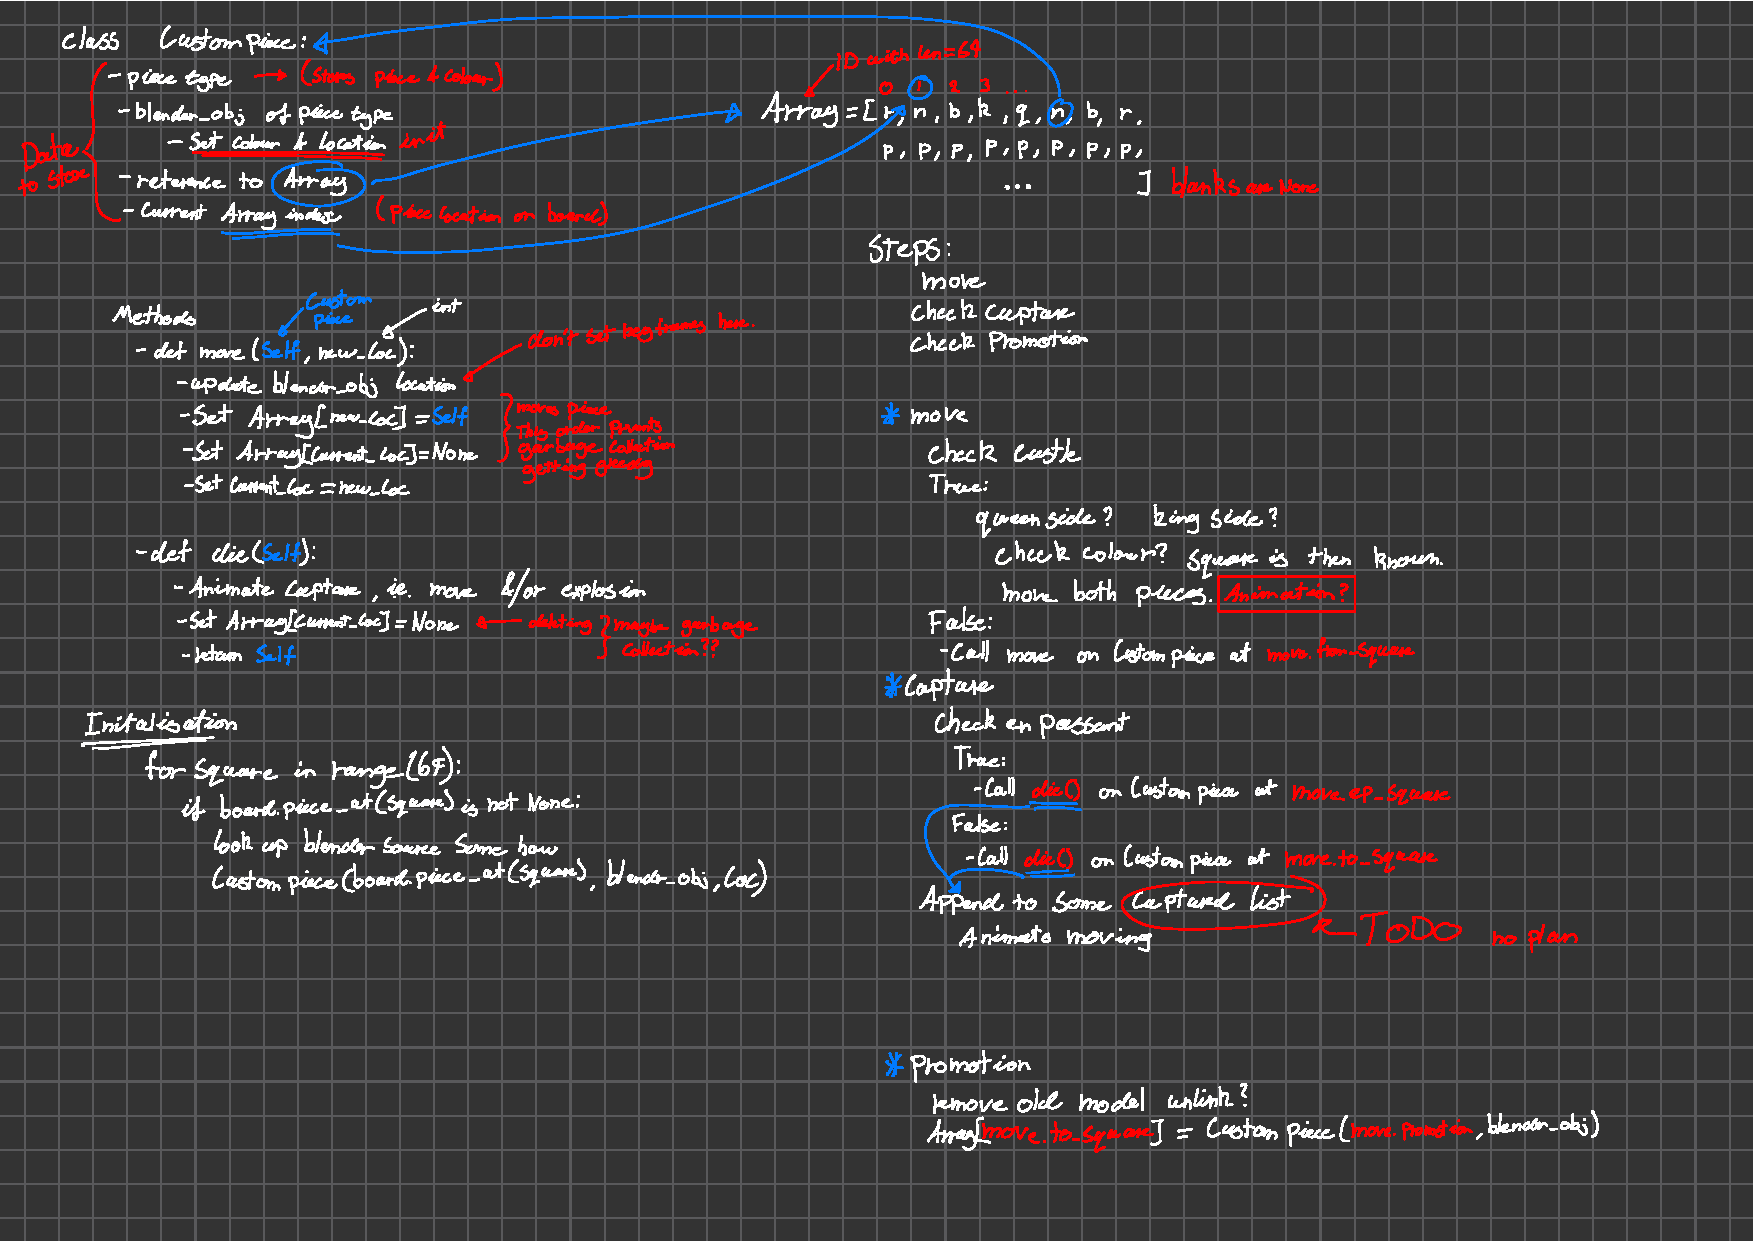
\includegraphics[width=\textwidth]{Scratchpad.pdf}
\caption{\label{class-sketch}\texttt{CustomPiece} Initial sketch}
\end{figure}

\begin{Code}
\begin{Verbatim}[]
\color[HTML]{383a42}\EFk{class} \EFt{CustomPiece}():
    \EFk{def} \EFf{\_\_init\_\_}(\EFk{self}, \EFv{pieceType}: chess.Piece, blender\_obj: bpy.types.Object,\char92{}
                 array: List[Optional[CustomPiece]], loc: \EFb{int}):
        \EFk{self}.\_pieceType = pieceType.piece\_type \EFcd{\# }\EFct{int}
        \EFk{self}.\EFv{\_colour} = pieceType.color         \EFcd{\# }\EFct{bool}
        \EFk{self}.\EFv{\_blender\_obj} = blender\_obj.copy()
        \EFk{self}.\EFv{\_array} = array                    \EFcd{\# }\EFct{reference to array containing self}
        \EFk{self}.\EFv{\_inital\_loc} = loc
        \EFk{self}.\EFv{\_loc} = loc                        \EFcd{\# }\EFct{int (1d array index)}

        \EFv{x}, \EFv{y} = square\_to\_world\_space(\EFk{self}.\_loc)
        \EFk{self}.\_blender\_obj.\EFv{location} = Vector((x, y, \EFhn{0.3}))

        \EFcd{\# }\EFct{set material based on colour}
        \EFk{if} \EFk{self}.\EFv{\_colour}:
            \EFk{self}.\_mat = bpy.data.materials[\EFs{"White pieces"}]
        \EFk{else}:
            \EFk{self}.\_mat = bpy.data.materials[\EFs{"Black pieces"}]
        \EFk{self}.\_blender\_obj.\EFv{active\_material} = \EFk{self}.\_mat


        \EFk{if} \EFk{self}.\_colour \EFk{and} \EFk{self}.\_pieceType == chess.KNIGHT:
            \EFk{self}.\_blender\_obj.rotation\_euler[\EFhn{2}] = radians(\EFhn{180}) \EFcd{\#}\EFct{XYZ}
        \EFcd{\# }\EFct{add object to collection so its visable}
        bpy.data.collections[[\EFs{'Black'}, \EFs{'White'}][\EFk{self}.\_colour]].objects.link(\EFk{self}.\_blender\_obj)

    \EFk{def} \EFf{move}(\EFk{self}, new\_loc: \EFb{int}, zTo: \EFb{float} = \EFhn{0.3}):
        \EFv{xTo}, \EFv{yTo} = square\_to\_world\_space(new\_loc)
        \EFk{self}.\_blender\_obj.location = Vector((xTo, yTo, zTo))
        \EFk{print}(\EFs{"Moved to "}, \EFk{self}.\_blender\_obj.location)

        \EFk{self}.\_array[\EFv{new\_loc}] = \EFk{self}
        \EFk{self}.\_array[\EFk{self}.\EFv{\_loc}] = \EFc{None}

        \EFk{self}.\_loc = new\_loc

    \EFk{def} \EFf{die}(\EFk{self}) -> CustomPiece:
        \EFk{self}.\_array[\EFk{self}.\EFv{\_loc}] = \EFc{None}
        \EFk{self}.keyframe\_insert(data\_path=\EFs{"location"}, frame=FRAME\_COUNT-\EFhn{6})

        \EFv{xTo}, \EFv{yTo} = square\_to\_world\_space(\EFk{self}.\_loc)
        \EFk{self}.\_blender\_obj.location = Vector((xTo, yTo, \EFhn{2.1}))
        \EFk{self}.keyframe\_insert(data\_path=\EFs{"location"}, frame=FRAME\_COUNT+\EFhn{3})

        \EFk{if} \EFk{self}.\_colour:
            \EFk{self}.\_inital\_loc += -\EFhn{16}
        \EFk{else}:
            \EFk{self}.\_inital\_loc += \EFhn{16}

        \EFv{xTo}, \EFv{yTo} = square\_to\_world\_space(\EFk{self}.\_inital\_loc)
        \EFk{self}.\_blender\_obj.location = Vector((xTo, yTo, \EFhn{2.1}))
        \EFk{self}.keyframe\_insert(data\_path=\EFs{"location"}, frame=FRAME\_COUNT+\EFhn{21})

        \EFv{xTo}, \EFv{yTo} = square\_to\_world\_space(\EFk{self}.\_inital\_loc)
        \EFk{self}.\_blender\_obj.location = Vector((xTo, yTo, \EFhn{0.1}))
        \EFk{self}.keyframe\_insert(data\_path=\EFs{"location"}, frame=FRAME\_COUNT+\EFhn{29})

        \EFk{return} \EFk{self}
\end{Verbatim}
\end{Code}
\label{class-src}

\newpage
\printbibliography
\end{document}
